\documentclass[twoside]{book}

% Packages required by doxygen
\usepackage{fixltx2e}
\usepackage{calc}
\usepackage{doxygen}
\usepackage[export]{adjustbox} % also loads graphicx
\usepackage{graphicx}
\usepackage[utf8]{inputenc}
\usepackage{makeidx}
\usepackage{multicol}
\usepackage{multirow}
\PassOptionsToPackage{warn}{textcomp}
\usepackage{textcomp}
\usepackage[nointegrals]{wasysym}
\usepackage[table]{xcolor}

% Font selection
\usepackage[T1]{fontenc}
\usepackage[scaled=.90]{helvet}
\usepackage{courier}
\usepackage{amssymb}
\usepackage{sectsty}
\renewcommand{\familydefault}{\sfdefault}
\allsectionsfont{%
  \fontseries{bc}\selectfont%
  \color{darkgray}%
}
\renewcommand{\DoxyLabelFont}{%
  \fontseries{bc}\selectfont%
  \color{darkgray}%
}
\newcommand{\+}{\discretionary{\mbox{\scriptsize$\hookleftarrow$}}{}{}}

% Page & text layout
\usepackage{geometry}
\geometry{%
  a4paper,%
  top=2.5cm,%
  bottom=2.5cm,%
  left=2.5cm,%
  right=2.5cm%
}
\tolerance=750
\hfuzz=15pt
\hbadness=750
\setlength{\emergencystretch}{15pt}
\setlength{\parindent}{0cm}
\setlength{\parskip}{3ex plus 2ex minus 2ex}
\makeatletter
\renewcommand{\paragraph}{%
  \@startsection{paragraph}{4}{0ex}{-1.0ex}{1.0ex}{%
    \normalfont\normalsize\bfseries\SS@parafont%
  }%
}
\renewcommand{\subparagraph}{%
  \@startsection{subparagraph}{5}{0ex}{-1.0ex}{1.0ex}{%
    \normalfont\normalsize\bfseries\SS@subparafont%
  }%
}
\makeatother

% Headers & footers
\usepackage{fancyhdr}
\pagestyle{fancyplain}
\fancyhead[LE]{\fancyplain{}{\bfseries\thepage}}
\fancyhead[CE]{\fancyplain{}{}}
\fancyhead[RE]{\fancyplain{}{\bfseries\leftmark}}
\fancyhead[LO]{\fancyplain{}{\bfseries\rightmark}}
\fancyhead[CO]{\fancyplain{}{}}
\fancyhead[RO]{\fancyplain{}{\bfseries\thepage}}
\fancyfoot[LE]{\fancyplain{}{}}
\fancyfoot[CE]{\fancyplain{}{}}
\fancyfoot[RE]{\fancyplain{}{\bfseries\scriptsize Generated by Doxygen }}
\fancyfoot[LO]{\fancyplain{}{\bfseries\scriptsize Generated by Doxygen }}
\fancyfoot[CO]{\fancyplain{}{}}
\fancyfoot[RO]{\fancyplain{}{}}
\renewcommand{\footrulewidth}{0.4pt}
\renewcommand{\chaptermark}[1]{%
  \markboth{#1}{}%
}
\renewcommand{\sectionmark}[1]{%
  \markright{\thesection\ #1}%
}

% Indices & bibliography
\usepackage{natbib}
\usepackage[titles]{tocloft}
\setcounter{tocdepth}{3}
\setcounter{secnumdepth}{5}
\makeindex

% Hyperlinks (required, but should be loaded last)
\usepackage{ifpdf}
\ifpdf
  \usepackage[pdftex,pagebackref=true]{hyperref}
\else
  \usepackage[ps2pdf,pagebackref=true]{hyperref}
\fi
\hypersetup{%
  colorlinks=true,%
  linkcolor=blue,%
  citecolor=blue,%
  unicode%
}

% Custom commands
\newcommand{\clearemptydoublepage}{%
  \newpage{\pagestyle{empty}\cleardoublepage}%
}

\usepackage{caption}
\captionsetup{labelsep=space,justification=centering,font={bf},singlelinecheck=off,skip=4pt,position=top}

%===== C O N T E N T S =====

\begin{document}

% Titlepage & ToC
\hypersetup{pageanchor=false,
             bookmarksnumbered=true,
             pdfencoding=unicode
            }
\pagenumbering{alph}
\begin{titlepage}
\vspace*{7cm}
\begin{center}%
{\Large Rad\+Map Analysis Framework }\\
\vspace*{1cm}
{\large Generated by Doxygen 1.8.13}\\
\end{center}
\end{titlepage}
\clearemptydoublepage
\pagenumbering{roman}
\tableofcontents
\clearemptydoublepage
\pagenumbering{arabic}
\hypersetup{pageanchor=true}

%--- Begin generated contents ---
\chapter{Install guide}
\label{md_README}
\Hypertarget{md_README}
\subsection*{Prerequisites}


\begin{DoxyItemize}
\item root
\item cmake
\end{DoxyItemize}

\subsection*{Installation}


\begin{DoxyEnumerate}
\item Go to your favorite destination
\item {\ttfamily git clone \href{https://github.com/tklemenz/RadMapAnalysis}{\tt https\+://github.\+com/tklemenz/\+Rad\+Map\+Analysis}}
\item source your {\ttfamily thisroot.\+sh}
\item {\ttfamily source Rad\+Map\+Analysis/compile.\+sh}
\item It\textquotesingle{}s that easy
\end{DoxyEnumerate}

\section*{How to use it}

When you want to open a root file containing objects from the framework you need to load the Rad\+Map\+Analysis.\+so (.dylib if you\textquotesingle{}re a mac disciple) library.

The easiest way I found for now is to create an alias in your {\ttfamily $\sim$/.bashrc} where the library is loaded when you call {\ttfamily root}. It could look something like this\+:

{\ttfamily alias rad\+R\+O\+OT=\textquotesingle{}root -\/l -\/e \char`\"{}g\+System-\/$>$\+Load(\textbackslash{}\char`\"{}/path/to/\+Rad\+Map\+Analysis/build/lib\+Rad\+Map\+Ana.so");"\textquotesingle{}}

Then you can simply call {\ttfamily rad\+R\+O\+OT} and the objects from the framework are known to root.

\section*{General stuff}


\begin{DoxyItemize}
\item compile.\+sh should not be changed!
\item Executables will be located in the bin folder.
\item As the only style guide I would suggest to N\+OT use tab but only spaces. Otherwise the code looks horrible in different editors...
\end{DoxyItemize}

Please only commit the following files or files in the following folders if changes were made (gitignore should take care of that)\+:


\begin{DoxyItemize}
\item C\+Make\+Lists.\+txt
\item include
\item src
\item macros
\item R\+E\+A\+D\+M\+E.\+md
\end{DoxyItemize}

Do N\+OT commit\+:


\begin{DoxyItemize}
\item bin
\item build
\end{DoxyItemize}

Feel free to not only add macros but also add missing functionality to the classes or create new classes that you think are necessary.

If you don\textquotesingle{}t know how to add classes and/or macros just go along the lines of the \hyperlink{classDummy}{Dummy} (add to Link\+Def and C\+Make\+Lists.\+txt etc...).

Thanks for contributing!! 
\chapter{Todo List}
\label{todo}
\Hypertarget{todo}

\begin{DoxyRefList}
\item[\label{todo__todo000001}%
\Hypertarget{todo__todo000001}%
Member \hyperlink{classCluster_aa12f4e548b102a48621ca7ec91bc2330}{Cluster\+:\+:add\+Signal} (const \hyperlink{classSignal}{Signal} \&signal)]Figure out how to properly calculate the sigmas of fiber and time\+Stamp  
\item[\label{todo__todo000002}%
\Hypertarget{todo__todo000002}%
Class \hyperlink{classTrack}{Track} ]Think about more info to be added to the track. E.\+g. angles, position (could be x-\/y in layer 1+2 and layer 3+4 separately) 
\end{DoxyRefList}
\chapter{Namespace Index}
\section{Namespace List}
Here is a list of all documented namespaces with brief descriptions\+:\begin{DoxyCompactList}
\item\contentsline{section}{\hyperlink{namespacemapping}{mapping} \\*This namespace holds the mapping functions }{\pageref{namespacemapping}}{}
\item\contentsline{section}{\hyperlink{namespacetext}{text} \\*This namespace holds some useless text modifications for terminal output }{\pageref{namespacetext}}{}
\end{DoxyCompactList}

\chapter{Hierarchical Index}
\section{Class Hierarchy}
This inheritance list is sorted roughly, but not completely, alphabetically\+:\begin{DoxyCompactList}
\item \contentsline{section}{Cluster}{\pageref{classCluster}}{}
\item \contentsline{section}{Clusterer}{\pageref{classClusterer}}{}
\item \contentsline{section}{Dummy}{\pageref{classDummy}}{}
\item \contentsline{section}{Event\+Base}{\pageref{classEventBase}}{}
\begin{DoxyCompactList}
\item \contentsline{section}{C\+T\+S\+Event}{\pageref{classCTSEvent}}{}
\item \contentsline{section}{C\+T\+S\+Event\+Clusters}{\pageref{classCTSEventClusters}}{}
\end{DoxyCompactList}
\item \contentsline{section}{Fiber}{\pageref{classFiber}}{}
\item \contentsline{section}{Module}{\pageref{classModule}}{}
\item \contentsline{section}{Signal}{\pageref{classSignal}}{}
\item \contentsline{section}{Track}{\pageref{classTrack}}{}
\item \contentsline{section}{Tracker}{\pageref{classTracker}}{}
\end{DoxyCompactList}

\chapter{Class Index}
\section{Class List}
Here are the classes, structs, unions and interfaces with brief descriptions\+:\begin{DoxyCompactList}
\item\contentsline{section}{\hyperlink{classCluster}{Cluster} }{\pageref{classCluster}}{}
\item\contentsline{section}{\hyperlink{classClusterer}{Clusterer} \\*\hyperlink{classClusterer}{Clusterer} class to assign signals from C\+T\+S\+Events to clusters }{\pageref{classClusterer}}{}
\item\contentsline{section}{\hyperlink{classCTSEvent}{C\+T\+S\+Event} }{\pageref{classCTSEvent}}{}
\item\contentsline{section}{\hyperlink{classCTSEventClusters}{C\+T\+S\+Event\+Clusters} }{\pageref{classCTSEventClusters}}{}
\item\contentsline{section}{\hyperlink{classDummy}{Dummy} }{\pageref{classDummy}}{}
\item\contentsline{section}{\hyperlink{classEventBase}{Event\+Base} }{\pageref{classEventBase}}{}
\item\contentsline{section}{\hyperlink{classFiber}{Fiber} }{\pageref{classFiber}}{}
\item\contentsline{section}{\hyperlink{classModule}{Module} }{\pageref{classModule}}{}
\item\contentsline{section}{\hyperlink{classSignal}{Signal} }{\pageref{classSignal}}{}
\item\contentsline{section}{\hyperlink{classTrack}{Track} }{\pageref{classTrack}}{}
\item\contentsline{section}{\hyperlink{classTracker}{Tracker} }{\pageref{classTracker}}{}
\end{DoxyCompactList}

\chapter{Namespace Documentation}
\hypertarget{namespacemapping}{}\section{mapping Namespace Reference}
\label{namespacemapping}\index{mapping@{mapping}}


This namespace holds the mapping functions.  


\subsection*{Functions}
\begin{DoxyCompactItemize}
\item 
std\+::pair$<$ Int\+\_\+t, Int\+\_\+t $>$ \hyperlink{namespacemapping_aa1474356b6c030e524bce7a388e20cd8}{get\+Fiber\+Info\+From\+Mod\+Spot} (Int\+\_\+t mod\+Spot)
\item 
\mbox{\Hypertarget{namespacemapping_a669c8c96499dd4cfc01a5fdf1bde8c41}\label{namespacemapping_a669c8c96499dd4cfc01a5fdf1bde8c41}} 
Int\+\_\+t \hyperlink{namespacemapping_a669c8c96499dd4cfc01a5fdf1bde8c41}{get\+Fiber\+Nr} (U\+Int\+\_\+t configuration, U\+Int\+\_\+t ch\+ID, U\+Int\+\_\+t tdc\+ID)
\begin{DoxyCompactList}\small\item\em get the fiber number within the layer from the padiwa configuration, channel ID, and T\+DC ID \end{DoxyCompactList}\item 
\mbox{\Hypertarget{namespacemapping_a43a9e5bffd76bc38c7db7eb18a6b70e0}\label{namespacemapping_a43a9e5bffd76bc38c7db7eb18a6b70e0}} 
Int\+\_\+t \hyperlink{namespacemapping_a43a9e5bffd76bc38c7db7eb18a6b70e0}{get\+Layer\+Nr} (U\+Int\+\_\+t configuration, U\+Int\+\_\+t ch\+ID, U\+Int\+\_\+t tdc\+ID)
\begin{DoxyCompactList}\small\item\em get the layer number from the padiwa configuration, channel ID, and T\+DC ID \end{DoxyCompactList}\item 
\mbox{\Hypertarget{namespacemapping_a02282299fd81a205ed060a81bdf12aaf}\label{namespacemapping_a02282299fd81a205ed060a81bdf12aaf}} 
Int\+\_\+t \hyperlink{namespacemapping_a02282299fd81a205ed060a81bdf12aaf}{getX} (Int\+\_\+t layer, Int\+\_\+t fiber)
\begin{DoxyCompactList}\small\item\em get the fiber number in x-\/direction from the fiber number and layer number. returns 0 for even layers. \end{DoxyCompactList}\item 
\mbox{\Hypertarget{namespacemapping_a24d3fe7e5b7af74cd5215d2930a5c877}\label{namespacemapping_a24d3fe7e5b7af74cd5215d2930a5c877}} 
Int\+\_\+t \hyperlink{namespacemapping_a24d3fe7e5b7af74cd5215d2930a5c877}{getY} (Int\+\_\+t layer, Int\+\_\+t fiber)
\begin{DoxyCompactList}\small\item\em get the fiber number in y-\/direction from the fiber number and layer number. returns 0 for odd layers. \end{DoxyCompactList}\item 
\mbox{\Hypertarget{namespacemapping_a4472aa4e6cd75914285a1c985c09b068}\label{namespacemapping_a4472aa4e6cd75914285a1c985c09b068}} 
Int\+\_\+t \hyperlink{namespacemapping_a4472aa4e6cd75914285a1c985c09b068}{get\+Module\+Spot} (Int\+\_\+t layer, Int\+\_\+t fiber)
\begin{DoxyCompactList}\small\item\em get the fiber number (0 -\/ 255) that the layer+fiber combination takes in the module \end{DoxyCompactList}\item 
U\+Int\+\_\+t \hyperlink{namespacemapping_a00520b73ed7ad6ada40fe422bf20b4b7}{odd0} (U\+Int\+\_\+t ch\+ID)
\item 
\mbox{\Hypertarget{namespacemapping_ada62caaf027acc96d2491da32de8ad07}\label{namespacemapping_ada62caaf027acc96d2491da32de8ad07}} 
U\+Int\+\_\+t {\bfseries odd1} (U\+Int\+\_\+t ch\+ID)
\item 
\mbox{\Hypertarget{namespacemapping_a64c663d1d62049966d0915d46abc55ba}\label{namespacemapping_a64c663d1d62049966d0915d46abc55ba}} 
U\+Int\+\_\+t {\bfseries rev\+Even0} (U\+Int\+\_\+t ch\+ID)
\item 
\mbox{\Hypertarget{namespacemapping_a363de8de2a9ea380113fbe5f8d68aa4a}\label{namespacemapping_a363de8de2a9ea380113fbe5f8d68aa4a}} 
U\+Int\+\_\+t {\bfseries rev\+Even1} (U\+Int\+\_\+t ch\+ID)
\item 
\mbox{\Hypertarget{namespacemapping_a3d99dd98372f99c279f77b9cfa250411}\label{namespacemapping_a3d99dd98372f99c279f77b9cfa250411}} 
Float\+\_\+t \hyperlink{namespacemapping_a3d99dd98372f99c279f77b9cfa250411}{get\+Coord} (Float\+\_\+t mean\+Fiber)
\begin{DoxyCompactList}\small\item\em get the actual spatial coordinate in mm \end{DoxyCompactList}\end{DoxyCompactItemize}


\subsection{Detailed Description}
This namespace holds the mapping functions. 

\subsection{Function Documentation}
\mbox{\Hypertarget{namespacemapping_aa1474356b6c030e524bce7a388e20cd8}\label{namespacemapping_aa1474356b6c030e524bce7a388e20cd8}} 
\index{mapping@{mapping}!get\+Fiber\+Info\+From\+Mod\+Spot@{get\+Fiber\+Info\+From\+Mod\+Spot}}
\index{get\+Fiber\+Info\+From\+Mod\+Spot@{get\+Fiber\+Info\+From\+Mod\+Spot}!mapping@{mapping}}
\subsubsection{\texorpdfstring{get\+Fiber\+Info\+From\+Mod\+Spot()}{getFiberInfoFromModSpot()}}
{\footnotesize\ttfamily std\+::pair$<$ Int\+\_\+t, Int\+\_\+t $>$ mapping\+::get\+Fiber\+Info\+From\+Mod\+Spot (\begin{DoxyParamCaption}\item[{Int\+\_\+t}]{mod\+Spot }\end{DoxyParamCaption})}

get the layer and fiber number from the module spot returns std\+::pair$<$layer,fiber$>$ $<$ 0 -\/ 31 --$>$ layer 1, fiber 1-\/32 32 -\/ 63 --$>$ layer 2, fiber 1-\/32 64 -\/ 95 --$>$ layer 3, fiber 1-\/32 96 -\/127 --$>$ layer 4, fiber 1-\/32 128 -\/159 --$>$ layer 5, fiber 1-\/32 160 -\/191 --$>$ layer 6, fiber 1-\/32 192 -\/223 --$>$ layer 7, fiber 1-\/32 224 -\/255 --$>$ layer 8, fiber 1-\/32 \mbox{\Hypertarget{namespacemapping_a00520b73ed7ad6ada40fe422bf20b4b7}\label{namespacemapping_a00520b73ed7ad6ada40fe422bf20b4b7}} 
\index{mapping@{mapping}!odd0@{odd0}}
\index{odd0@{odd0}!mapping@{mapping}}
\subsubsection{\texorpdfstring{odd0()}{odd0()}}
{\footnotesize\ttfamily U\+Int\+\_\+t mapping\+::odd0 (\begin{DoxyParamCaption}\item[{U\+Int\+\_\+t}]{ch\+ID }\end{DoxyParamCaption})\hspace{0.3cm}{\ttfamily [inline]}}

mapping functions from channel number to fiber odd maps channel number to odd numbers from 1-\/31 rev\+Even maps channel number to even numbers from 32-\/2 0 is for channel number 1-\/16 1 is for channel number 17-\/32 
\hypertarget{namespacetext}{}\section{text Namespace Reference}
\label{namespacetext}\index{text@{text}}


This namespace holds some useless text modifications for terminal output.  


\subsection*{Variables}
\begin{DoxyCompactItemize}
\item 
\mbox{\Hypertarget{namespacetext_a4fa213f28668cba2af5bde1d3d7904df}\label{namespacetext_a4fa213f28668cba2af5bde1d3d7904df}} 
const char $\ast$const {\bfseries B\+LK} = \char`\"{}\textbackslash{}e\mbox{[}30m\char`\"{}
\item 
\mbox{\Hypertarget{namespacetext_ac2e454d781dce06ac89c972d0f999fb8}\label{namespacetext_ac2e454d781dce06ac89c972d0f999fb8}} 
const char $\ast$const {\bfseries R\+ED} = \char`\"{}\textbackslash{}e\mbox{[}31m\char`\"{}
\item 
\mbox{\Hypertarget{namespacetext_a6c5120d8850011f6cb2c121366feb6e4}\label{namespacetext_a6c5120d8850011f6cb2c121366feb6e4}} 
const char $\ast$const {\bfseries G\+RN} = \char`\"{}\textbackslash{}e\mbox{[}32m\char`\"{}
\item 
\mbox{\Hypertarget{namespacetext_af5249403cb35818689a627c7ef57fae8}\label{namespacetext_af5249403cb35818689a627c7ef57fae8}} 
const char $\ast$const {\bfseries Y\+EL} = \char`\"{}\textbackslash{}e\mbox{[}33m\char`\"{}
\item 
\mbox{\Hypertarget{namespacetext_a84534480435c2964850e8fefad365754}\label{namespacetext_a84534480435c2964850e8fefad365754}} 
const char $\ast$const {\bfseries B\+LU} = \char`\"{}\textbackslash{}e\mbox{[}34m\char`\"{}
\item 
\mbox{\Hypertarget{namespacetext_ad29616145caa863968fc139e20aac10d}\label{namespacetext_ad29616145caa863968fc139e20aac10d}} 
const char $\ast$const {\bfseries M\+AG} = \char`\"{}\textbackslash{}e\mbox{[}35m\char`\"{}
\item 
\mbox{\Hypertarget{namespacetext_a5b68a851d3702a1c5589b552b0fd9bf8}\label{namespacetext_a5b68a851d3702a1c5589b552b0fd9bf8}} 
const char $\ast$const {\bfseries C\+YN} = \char`\"{}\textbackslash{}e\mbox{[}36m\char`\"{}
\item 
\mbox{\Hypertarget{namespacetext_ad2a49861a124ccdf50f7fc852c323552}\label{namespacetext_ad2a49861a124ccdf50f7fc852c323552}} 
const char $\ast$const {\bfseries G\+RY} = \char`\"{}\textbackslash{}e\mbox{[}37m\char`\"{}
\item 
\mbox{\Hypertarget{namespacetext_a6f9b75ab7ce9cf6568ff22ff150c06d9}\label{namespacetext_a6f9b75ab7ce9cf6568ff22ff150c06d9}} 
const char $\ast$const {\bfseries L\+B\+LK} = \char`\"{}\textbackslash{}e\mbox{[}90m\char`\"{}
\item 
\mbox{\Hypertarget{namespacetext_a1f30bd6fafff687ab2035f1bb00b42e1}\label{namespacetext_a1f30bd6fafff687ab2035f1bb00b42e1}} 
const char $\ast$const {\bfseries L\+R\+ED} = \char`\"{}\textbackslash{}e\mbox{[}91m\char`\"{}
\item 
\mbox{\Hypertarget{namespacetext_a872069935024fec17ce88c4e556454db}\label{namespacetext_a872069935024fec17ce88c4e556454db}} 
const char $\ast$const {\bfseries L\+G\+RN} = \char`\"{}\textbackslash{}e\mbox{[}92m\char`\"{}
\item 
\mbox{\Hypertarget{namespacetext_acff2282e0f020cf98df6859daf30fdad}\label{namespacetext_acff2282e0f020cf98df6859daf30fdad}} 
const char $\ast$const {\bfseries L\+Y\+EL} = \char`\"{}\textbackslash{}e\mbox{[}93m\char`\"{}
\item 
\mbox{\Hypertarget{namespacetext_a147548c2509e9d2ce000436678080a2a}\label{namespacetext_a147548c2509e9d2ce000436678080a2a}} 
const char $\ast$const {\bfseries L\+B\+LU} = \char`\"{}\textbackslash{}e\mbox{[}94m\char`\"{}
\item 
\mbox{\Hypertarget{namespacetext_a4efa2a831ca181ff54444e263d3672e8}\label{namespacetext_a4efa2a831ca181ff54444e263d3672e8}} 
const char $\ast$const {\bfseries L\+M\+AG} = \char`\"{}\textbackslash{}e\mbox{[}95m\char`\"{}
\item 
\mbox{\Hypertarget{namespacetext_ab2efc54c7cbf67c20705d0d901544c9b}\label{namespacetext_ab2efc54c7cbf67c20705d0d901544c9b}} 
const char $\ast$const {\bfseries L\+C\+YN} = \char`\"{}\textbackslash{}e\mbox{[}96m\char`\"{}
\item 
\mbox{\Hypertarget{namespacetext_af13bba2229e857161ccc0cdcd64ba998}\label{namespacetext_af13bba2229e857161ccc0cdcd64ba998}} 
const char $\ast$const {\bfseries W\+HT} = \char`\"{}\textbackslash{}e\mbox{[}97m\char`\"{}
\item 
\mbox{\Hypertarget{namespacetext_a2fd1a21b772940b61ef49d056bd473f4}\label{namespacetext_a2fd1a21b772940b61ef49d056bd473f4}} 
const char $\ast$const {\bfseries R\+E\+S\+ET} = \char`\"{}\textbackslash{}e\mbox{[}0m\char`\"{}
\item 
\mbox{\Hypertarget{namespacetext_a97dc4df776bd9db6064159997386b0e5}\label{namespacetext_a97dc4df776bd9db6064159997386b0e5}} 
const char $\ast$const {\bfseries B\+O\+LD} = \char`\"{}\textbackslash{}e\mbox{[}1m\char`\"{}
\item 
\mbox{\Hypertarget{namespacetext_a7bf854af552237d9c8e3a422b9dabcc5}\label{namespacetext_a7bf854af552237d9c8e3a422b9dabcc5}} 
const char $\ast$const {\bfseries U\+L\+I\+NE} = \char`\"{}\textbackslash{}e\mbox{[}4m\char`\"{}
\item 
\mbox{\Hypertarget{namespacetext_a224cbea063847abbb2d57eb0eeb7e969}\label{namespacetext_a224cbea063847abbb2d57eb0eeb7e969}} 
const char $\ast$const {\bfseries B\+L\+I\+NK} = \char`\"{}\textbackslash{}e\mbox{[}5m\char`\"{}
\end{DoxyCompactItemize}


\subsection{Detailed Description}
This namespace holds some useless text modifications for terminal output. 
\chapter{Class Documentation}
\hypertarget{classCluster}{}\section{Cluster Class Reference}
\label{classCluster}\index{Cluster@{Cluster}}


{\ttfamily \#include $<$Cluster.\+h$>$}

\subsection*{Public Types}
\begin{DoxyCompactItemize}
\item 
enum \hyperlink{classCluster_a161820c1803e25a96fb5075c63828451}{Flags} \+: unsigned short \{ \hyperlink{classCluster_a161820c1803e25a96fb5075c63828451a07b5d8988299b30135aecdb9cf48d0c5}{used\+In\+Track} = 0x1 $<$$<$ 0
 \}
\end{DoxyCompactItemize}
\subsection*{Public Member Functions}
\begin{DoxyCompactItemize}
\item 
\mbox{\Hypertarget{classCluster_a115edd51ef79406194cfa10ad5f44688}\label{classCluster_a115edd51ef79406194cfa10ad5f44688}} 
\hyperlink{classCluster_a115edd51ef79406194cfa10ad5f44688}{Cluster} ()=default
\begin{DoxyCompactList}\small\item\em default constructor \end{DoxyCompactList}\item 
\mbox{\Hypertarget{classCluster_a0dae97c5173ed13d405a8cf5b03dc497}\label{classCluster_a0dae97c5173ed13d405a8cf5b03dc497}} 
\hyperlink{classCluster_a0dae97c5173ed13d405a8cf5b03dc497}{$\sim$\+Cluster} ()=default
\begin{DoxyCompactList}\small\item\em default destructor \end{DoxyCompactList}\item 
\mbox{\Hypertarget{classCluster_aee67361b05ff006a0a90e87c712cc338}\label{classCluster_aee67361b05ff006a0a90e87c712cc338}} 
\hyperlink{classCluster_aee67361b05ff006a0a90e87c712cc338}{Cluster} (const \hyperlink{classCluster}{Cluster} \&cluster)
\begin{DoxyCompactList}\small\item\em Copy constructor. \end{DoxyCompactList}\item 
\mbox{\Hypertarget{classCluster_a64840fa60acf13c89406a38c1475014c}\label{classCluster_a64840fa60acf13c89406a38c1475014c}} 
\hyperlink{classCluster_a64840fa60acf13c89406a38c1475014c}{Cluster} (const Double\+\_\+t q\+Tot, const Double\+\_\+t q\+Max, const Float\+\_\+t mean\+Fiber, const Float\+\_\+t sigma\+Fiber, const Double\+\_\+t mean\+Time\+Stamp, const Double\+\_\+t sigma\+Time\+Stamp, const Double\+\_\+t first\+Time\+Stamp, const Int\+\_\+t layer, const Int\+\_\+t T\+D\+C\+ID, const Short\+\_\+t flags)
\begin{DoxyCompactList}\small\item\em This constructor should be used in most cases. It takes all \hyperlink{classCluster}{Cluster} information. \end{DoxyCompactList}\item 
\mbox{\Hypertarget{classCluster_a3fb10af0d537659bc85844087dbdb5d2}\label{classCluster_a3fb10af0d537659bc85844087dbdb5d2}} 
bool \hyperlink{classCluster_a3fb10af0d537659bc85844087dbdb5d2}{is\+Used} () const
\begin{DoxyCompactList}\small\item\em Check if the Clsuter was already associated to a \hyperlink{classTrack}{Track}. \end{DoxyCompactList}\item 
\mbox{\Hypertarget{classCluster_a5d893796dabaaf60c0ae1ad59df90f29}\label{classCluster_a5d893796dabaaf60c0ae1ad59df90f29}} 
void \hyperlink{classCluster_a5d893796dabaaf60c0ae1ad59df90f29}{set\+Is\+Used} ()
\begin{DoxyCompactList}\small\item\em Set the used\+In\+Track flag for the \hyperlink{classTracker}{Tracker}. \end{DoxyCompactList}\item 
\mbox{\Hypertarget{classCluster_a2cb9837dc7527521adbbfd004e5ab638}\label{classCluster_a2cb9837dc7527521adbbfd004e5ab638}} 
void {\bfseries set\+Q\+Tot} (Double\+\_\+t \&q\+Tot)
\item 
\mbox{\Hypertarget{classCluster_acba72d0c451b429ac1ae8f0fef46ac83}\label{classCluster_acba72d0c451b429ac1ae8f0fef46ac83}} 
void {\bfseries set\+Q\+Max} (Double\+\_\+t \&q\+Max)
\item 
\mbox{\Hypertarget{classCluster_a181d1faa8d3d0bda8424bebe868d13ac}\label{classCluster_a181d1faa8d3d0bda8424bebe868d13ac}} 
void {\bfseries set\+Mean\+Fiber} (Float\+\_\+t \&mean\+Fiber)
\item 
\mbox{\Hypertarget{classCluster_a8233157f8c83330a859fd0af284d36ad}\label{classCluster_a8233157f8c83330a859fd0af284d36ad}} 
void {\bfseries set\+Sigma\+Fiber} (Float\+\_\+t \&sigma\+Fiber)
\item 
\mbox{\Hypertarget{classCluster_acfa5cb90b8f6454dc757842c1e5921dc}\label{classCluster_acfa5cb90b8f6454dc757842c1e5921dc}} 
void {\bfseries set\+Mean\+Time\+Stamp} (Double\+\_\+t \&mean\+Time\+Stamp)
\item 
\mbox{\Hypertarget{classCluster_a7fa652aa68dec8e0148ce7f27ab79572}\label{classCluster_a7fa652aa68dec8e0148ce7f27ab79572}} 
void {\bfseries set\+Sigma\+Time\+Stamp} (Double\+\_\+t \&sigma\+Time\+Stamp)
\item 
\mbox{\Hypertarget{classCluster_aa5aad7f1fa30683814e404dead7eb59b}\label{classCluster_aa5aad7f1fa30683814e404dead7eb59b}} 
void {\bfseries set\+First\+Time\+Stamp} (Double\+\_\+t \&first\+Time\+Stamp)
\item 
\mbox{\Hypertarget{classCluster_ad4f4eb5d2636ca90754d77e1aebd1e61}\label{classCluster_ad4f4eb5d2636ca90754d77e1aebd1e61}} 
void {\bfseries set\+Layer} (Int\+\_\+t \&layer)
\item 
\mbox{\Hypertarget{classCluster_a69ecb0377864d4c9229c3dd9ab7576d0}\label{classCluster_a69ecb0377864d4c9229c3dd9ab7576d0}} 
void {\bfseries set\+T\+D\+C\+ID} (Int\+\_\+t \&tdc\+ID)
\item 
\mbox{\Hypertarget{classCluster_a480632337fcaf7629f8ba2490819cc9a}\label{classCluster_a480632337fcaf7629f8ba2490819cc9a}} 
Double\+\_\+t {\bfseries get\+Q\+Tot} ()
\item 
\mbox{\Hypertarget{classCluster_a1c5bc215c52e4bad5409fc09a8ca5865}\label{classCluster_a1c5bc215c52e4bad5409fc09a8ca5865}} 
Double\+\_\+t {\bfseries get\+Q\+Max} ()
\item 
\mbox{\Hypertarget{classCluster_afeea4a9ed002eea5f7b4d315adc2c537}\label{classCluster_afeea4a9ed002eea5f7b4d315adc2c537}} 
Float\+\_\+t {\bfseries get\+Mean\+Fiber} ()
\item 
\mbox{\Hypertarget{classCluster_aff40b7e0a9ca61d13b4914b93545eec2}\label{classCluster_aff40b7e0a9ca61d13b4914b93545eec2}} 
Float\+\_\+t {\bfseries get\+Sigma\+Fiber} ()
\item 
\mbox{\Hypertarget{classCluster_adbaa8320c05b9d1eeb5045becac00697}\label{classCluster_adbaa8320c05b9d1eeb5045becac00697}} 
Double\+\_\+t {\bfseries get\+Mean\+Time\+Stamp} ()
\item 
\mbox{\Hypertarget{classCluster_a0939ece440966900a066bbb950c09362}\label{classCluster_a0939ece440966900a066bbb950c09362}} 
Double\+\_\+t {\bfseries get\+Sigma\+Time\+Stamp} ()
\item 
\mbox{\Hypertarget{classCluster_a4c4d763ac24966aaac2bfb4591eb774e}\label{classCluster_a4c4d763ac24966aaac2bfb4591eb774e}} 
Double\+\_\+t {\bfseries get\+First\+Time\+Stamp} ()
\item 
\mbox{\Hypertarget{classCluster_af3d84b8a21a41f49ff292698eb0029d9}\label{classCluster_af3d84b8a21a41f49ff292698eb0029d9}} 
Int\+\_\+t {\bfseries get\+Layer} ()
\item 
\mbox{\Hypertarget{classCluster_ae38ce6e3bd38f4d8fd0c438be15640aa}\label{classCluster_ae38ce6e3bd38f4d8fd0c438be15640aa}} 
Int\+\_\+t {\bfseries get\+T\+D\+C\+ID} ()
\item 
void \hyperlink{classCluster_aa12f4e548b102a48621ca7ec91bc2330}{add\+Signal} (const \hyperlink{classSignal}{Signal} \&signal)
\item 
\mbox{\Hypertarget{classCluster_af2a12e41d81b74a04aa88c691b4c5c5b}\label{classCluster_af2a12e41d81b74a04aa88c691b4c5c5b}} 
Int\+\_\+t \hyperlink{classCluster_af2a12e41d81b74a04aa88c691b4c5c5b}{get\+N\+Signals} ()
\begin{DoxyCompactList}\small\item\em get the overall number of signals in the cluster \end{DoxyCompactList}\item 
\mbox{\Hypertarget{classCluster_ac76ad4f0d6b3db83e39364063e864a0c}\label{classCluster_ac76ad4f0d6b3db83e39364063e864a0c}} 
std\+::vector$<$ \hyperlink{classSignal}{Signal} $>$ \& \hyperlink{classCluster_ac76ad4f0d6b3db83e39364063e864a0c}{get\+Signals} ()
\begin{DoxyCompactList}\small\item\em returns the vector containing the signals in the cluster \end{DoxyCompactList}\end{DoxyCompactItemize}


\subsection{Detailed Description}
! This class represents a cluster of signals. Clusters consist of signals in neighboring fibers that stem from the same particle. The idea is to initialize a cluster object and call the function add\+Signal for every signal that shall be included in the cluster. 

\subsection{Member Enumeration Documentation}
\mbox{\Hypertarget{classCluster_a161820c1803e25a96fb5075c63828451}\label{classCluster_a161820c1803e25a96fb5075c63828451}} 
\index{Cluster@{Cluster}!Flags@{Flags}}
\index{Flags@{Flags}!Cluster@{Cluster}}
\subsubsection{\texorpdfstring{Flags}{Flags}}
{\footnotesize\ttfamily enum \hyperlink{classCluster_a161820c1803e25a96fb5075c63828451}{Cluster\+::\+Flags} \+: unsigned short}

\begin{DoxyEnumFields}{Enumerator}
\raisebox{\heightof{T}}[0pt][0pt]{\index{used\+In\+Track@{used\+In\+Track}!Cluster@{Cluster}}\index{Cluster@{Cluster}!used\+In\+Track@{used\+In\+Track}}}\mbox{\Hypertarget{classCluster_a161820c1803e25a96fb5075c63828451a07b5d8988299b30135aecdb9cf48d0c5}\label{classCluster_a161820c1803e25a96fb5075c63828451a07b5d8988299b30135aecdb9cf48d0c5}} 
used\+In\+Track&Check if the \hyperlink{classCluster}{Cluster} is already associated to a \hyperlink{classTrack}{Track}. \\
\hline

\end{DoxyEnumFields}


\subsection{Member Function Documentation}
\mbox{\Hypertarget{classCluster_aa12f4e548b102a48621ca7ec91bc2330}\label{classCluster_aa12f4e548b102a48621ca7ec91bc2330}} 
\index{Cluster@{Cluster}!add\+Signal@{add\+Signal}}
\index{add\+Signal@{add\+Signal}!Cluster@{Cluster}}
\subsubsection{\texorpdfstring{add\+Signal()}{addSignal()}}
{\footnotesize\ttfamily void Cluster\+::add\+Signal (\begin{DoxyParamCaption}\item[{const \hyperlink{classSignal}{Signal} \&}]{signal }\end{DoxyParamCaption})\hspace{0.3cm}{\ttfamily [inline]}}

add a signal to the cluster calculates all cluster properties and updates members 
\begin{DoxyParams}{Parameters}
{\em \hyperlink{classSignal}{Signal}} & \\
\hline
\end{DoxyParams}
\begin{DoxyRefDesc}{Todo}
\item[\hyperlink{todo__todo000001}{Todo}]Figure out how to properly calculate the sigmas of fiber and time\+Stamp \end{DoxyRefDesc}


The documentation for this class was generated from the following files\+:\begin{DoxyCompactItemize}
\item 
Cluster.\+h\item 
Cluster.\+cxx\end{DoxyCompactItemize}

\hypertarget{classClusterer}{}\section{Clusterer Class Reference}
\label{classClusterer}\index{Clusterer@{Clusterer}}


\hyperlink{classClusterer}{Clusterer} class to assign signals from C\+T\+S\+Events to clusters.  




{\ttfamily \#include $<$Clusterer.\+h$>$}



\subsection{Detailed Description}
\hyperlink{classClusterer}{Clusterer} class to assign signals from C\+T\+S\+Events to clusters. 

The documentation for this class was generated from the following file\+:\begin{DoxyCompactItemize}
\item 
Clusterer.\+h\end{DoxyCompactItemize}

\hypertarget{classCTSEvent}{}\section{C\+T\+S\+Event Class Reference}
\label{classCTSEvent}\index{C\+T\+S\+Event@{C\+T\+S\+Event}}


{\ttfamily \#include $<$C\+T\+S\+Event.\+h$>$}



Inheritance diagram for C\+T\+S\+Event\+:\nopagebreak
\begin{figure}[H]
\begin{center}
\leavevmode
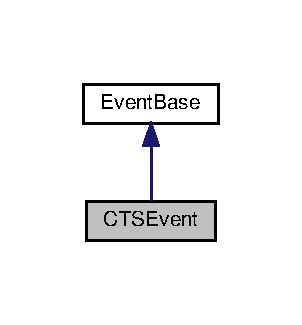
\includegraphics[width=145pt]{classCTSEvent__inherit__graph}
\end{center}
\end{figure}


Collaboration diagram for C\+T\+S\+Event\+:\nopagebreak
\begin{figure}[H]
\begin{center}
\leavevmode
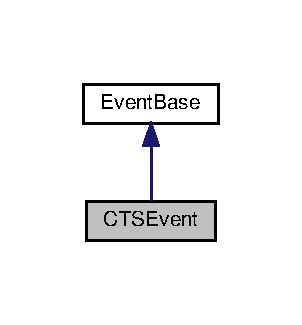
\includegraphics[width=145pt]{classCTSEvent__coll__graph}
\end{center}
\end{figure}
\subsection*{Public Member Functions}
\begin{DoxyCompactItemize}
\item 
\mbox{\Hypertarget{classCTSEvent_a9635121dd317e3a1f2c9dce8e8a62970}\label{classCTSEvent_a9635121dd317e3a1f2c9dce8e8a62970}} 
{\bfseries C\+T\+S\+Event} (const \hyperlink{classCTSEvent}{C\+T\+S\+Event} \&event)
\item 
\mbox{\Hypertarget{classCTSEvent_a681a21060ad13d5843509989be2c345d}\label{classCTSEvent_a681a21060ad13d5843509989be2c345d}} 
void {\bfseries set\+Module} (\hyperlink{classModule}{Module} \&module)
\item 
\mbox{\Hypertarget{classCTSEvent_a19b2ee23f6334def487ba09fc50af858}\label{classCTSEvent_a19b2ee23f6334def487ba09fc50af858}} 
\hyperlink{classModule}{Module} \& {\bfseries get\+Module} ()
\item 
\mbox{\Hypertarget{classCTSEvent_a0f2195c2a65119e85b4cfc3a1bf72c0f}\label{classCTSEvent_a0f2195c2a65119e85b4cfc3a1bf72c0f}} 
const \hyperlink{classModule}{Module} \& {\bfseries get\+Module} () const
\end{DoxyCompactItemize}


\subsection{Detailed Description}
This class represents a basic C\+TS event containing signals.

The module object contains all signal information.

Before an event is written to file the remove\+Empty funtion should be called on the module to reduce data size and increase performance. 

The documentation for this class was generated from the following files\+:\begin{DoxyCompactItemize}
\item 
C\+T\+S\+Event.\+h\item 
C\+T\+S\+Event.\+cxx\end{DoxyCompactItemize}

\hypertarget{classCTSEventClusters}{}\section{C\+T\+S\+Event\+Clusters Class Reference}
\label{classCTSEventClusters}\index{C\+T\+S\+Event\+Clusters@{C\+T\+S\+Event\+Clusters}}


{\ttfamily \#include $<$C\+T\+S\+Event\+Clusters.\+h$>$}



Inheritance diagram for C\+T\+S\+Event\+Clusters\+:\nopagebreak
\begin{figure}[H]
\begin{center}
\leavevmode
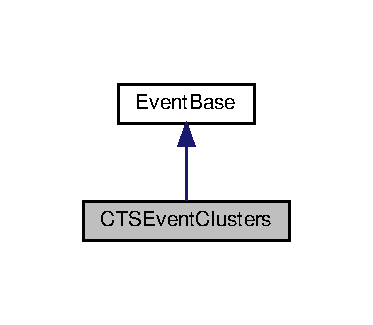
\includegraphics[width=179pt]{classCTSEventClusters__inherit__graph}
\end{center}
\end{figure}


Collaboration diagram for C\+T\+S\+Event\+Clusters\+:\nopagebreak
\begin{figure}[H]
\begin{center}
\leavevmode
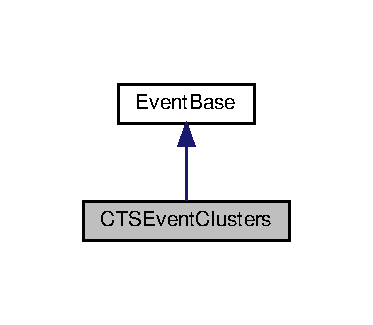
\includegraphics[width=179pt]{classCTSEventClusters__coll__graph}
\end{center}
\end{figure}
\subsection*{Public Member Functions}
\begin{DoxyCompactItemize}
\item 
\mbox{\Hypertarget{classCTSEventClusters_aa9ea39617fef98537e5f997052138e74}\label{classCTSEventClusters_aa9ea39617fef98537e5f997052138e74}} 
{\bfseries C\+T\+S\+Event\+Clusters} (const \hyperlink{classCTSEventClusters}{C\+T\+S\+Event\+Clusters} \&event)
\item 
\mbox{\Hypertarget{classCTSEventClusters_a6c0b9fb135b957df0f907a1f32f27ec1}\label{classCTSEventClusters_a6c0b9fb135b957df0f907a1f32f27ec1}} 
void {\bfseries add\+Cluster} (\hyperlink{classCluster}{Cluster} \&cluster)
\item 
\mbox{\Hypertarget{classCTSEventClusters_a885d19a07e71bb3e91b488449af10b5c}\label{classCTSEventClusters_a885d19a07e71bb3e91b488449af10b5c}} 
std\+::vector$<$ \hyperlink{classCluster}{Cluster} $>$ \& {\bfseries get\+Clusters} ()
\item 
\mbox{\Hypertarget{classCTSEventClusters_a405d7e8bad65c7371fd4855aaebfce84}\label{classCTSEventClusters_a405d7e8bad65c7371fd4855aaebfce84}} 
const std\+::vector$<$ \hyperlink{classCluster}{Cluster} $>$ \& {\bfseries get\+Clusters} () const
\end{DoxyCompactItemize}


\subsection{Detailed Description}
This class represents a C\+TS event containing clusters. It holds\+:
\begin{DoxyItemize}
\item a vector containing all clusters in the event 
\end{DoxyItemize}

The documentation for this class was generated from the following files\+:\begin{DoxyCompactItemize}
\item 
C\+T\+S\+Event\+Clusters.\+h\item 
C\+T\+S\+Event\+Clusters.\+cxx\end{DoxyCompactItemize}

\hypertarget{classDummy}{}\section{Dummy Class Reference}
\label{classDummy}\index{Dummy@{Dummy}}
\subsection*{Public Member Functions}
\begin{DoxyCompactItemize}
\item 
\mbox{\Hypertarget{classDummy_aaed3afdeb98915dd70a81f2d78c65f54}\label{classDummy_aaed3afdeb98915dd70a81f2d78c65f54}} 
{\bfseries Dummy} (const \hyperlink{classDummy}{Dummy} \&dummy)
\item 
\mbox{\Hypertarget{classDummy_aaad1dd5a6eaa48f6a475c361713b9b96}\label{classDummy_aaad1dd5a6eaa48f6a475c361713b9b96}} 
void {\bfseries set\+Member} (Int\+\_\+t value)
\item 
\mbox{\Hypertarget{classDummy_adfc4d409a0c41d424fc0ea0248930a27}\label{classDummy_adfc4d409a0c41d424fc0ea0248930a27}} 
Int\+\_\+t {\bfseries get\+Member} () const
\end{DoxyCompactItemize}


The documentation for this class was generated from the following files\+:\begin{DoxyCompactItemize}
\item 
Dummy.\+h\item 
Dummy.\+cxx\end{DoxyCompactItemize}

\hypertarget{classEventBase}{}\section{Event\+Base Class Reference}
\label{classEventBase}\index{Event\+Base@{Event\+Base}}


{\ttfamily \#include $<$Event\+Base.\+h$>$}



Inheritance diagram for Event\+Base\+:\nopagebreak
\begin{figure}[H]
\begin{center}
\leavevmode
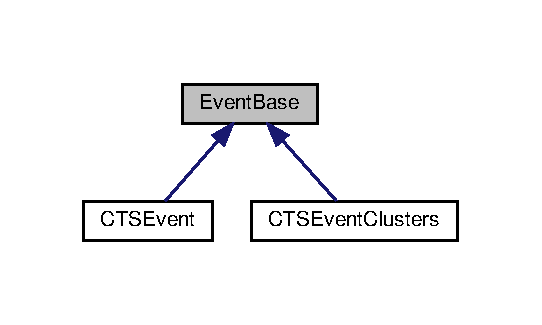
\includegraphics[width=260pt]{classEventBase__inherit__graph}
\end{center}
\end{figure}
\subsection*{Public Member Functions}
\begin{DoxyCompactItemize}
\item 
\mbox{\Hypertarget{classEventBase_a7451d4e0fe0969ccb386580c532ae840}\label{classEventBase_a7451d4e0fe0969ccb386580c532ae840}} 
{\bfseries Event\+Base} (const \hyperlink{classEventBase}{Event\+Base} \&event)
\item 
\mbox{\Hypertarget{classEventBase_a8a10415e840424b7f8c8e40ecea2b391}\label{classEventBase_a8a10415e840424b7f8c8e40ecea2b391}} 
void {\bfseries set\+Event\+Nr} (Float\+\_\+t event\+Nr)
\item 
\mbox{\Hypertarget{classEventBase_ac94ea2e36812d76b63e2ad0798fb85cc}\label{classEventBase_ac94ea2e36812d76b63e2ad0798fb85cc}} 
void {\bfseries set\+Padiwa\+Config} (Int\+\_\+t config)
\item 
\mbox{\Hypertarget{classEventBase_ae00e0bf9992a8c62d6f236bb01f7a785}\label{classEventBase_ae00e0bf9992a8c62d6f236bb01f7a785}} 
Float\+\_\+t {\bfseries get\+Event\+Nr} () const
\item 
\mbox{\Hypertarget{classEventBase_ae31520fb8359882ec91aeb7825f3e6e0}\label{classEventBase_ae31520fb8359882ec91aeb7825f3e6e0}} 
Int\+\_\+t {\bfseries get\+Padiwa\+Config} () const
\end{DoxyCompactItemize}


\subsection{Detailed Description}
This class represents a basic event from which specified event classes (e.\+g. \hyperlink{classCTSEvent}{C\+T\+S\+Event} or physical event classes) can be derived.

The philosophy still needs a bit of thought... The basic information the event holds is\+:
\begin{DoxyItemize}
\item Event\+Nr
\item Padiwa\+Config 
\end{DoxyItemize}

The documentation for this class was generated from the following file\+:\begin{DoxyCompactItemize}
\item 
Event\+Base.\+h\end{DoxyCompactItemize}

\hypertarget{classFiber}{}\section{Fiber Class Reference}
\label{classFiber}\index{Fiber@{Fiber}}


{\ttfamily \#include $<$Fiber.\+h$>$}

\subsection*{Public Member Functions}
\begin{DoxyCompactItemize}
\item 
\mbox{\Hypertarget{classFiber_ad2e469dbbb1c7ff0d08d8a451fe099da}\label{classFiber_ad2e469dbbb1c7ff0d08d8a451fe099da}} 
{\bfseries Fiber} (const \hyperlink{classFiber}{Fiber} \&fiber)
\item 
\mbox{\Hypertarget{classFiber_a82dec1d501c2bea3254d1e349e968a39}\label{classFiber_a82dec1d501c2bea3254d1e349e968a39}} 
{\bfseries Fiber} (const Int\+\_\+t layer, const Int\+\_\+t x, const Int\+\_\+t y)
\item 
\mbox{\Hypertarget{classFiber_aeed749f11255081384ec0f41793aa5de}\label{classFiber_aeed749f11255081384ec0f41793aa5de}} 
void {\bfseries set\+Layer} (Int\+\_\+t layer)
\item 
\mbox{\Hypertarget{classFiber_a14500d45eb679b65ee279118f1d9d585}\label{classFiber_a14500d45eb679b65ee279118f1d9d585}} 
void {\bfseries setX} (Int\+\_\+t x)
\item 
\mbox{\Hypertarget{classFiber_ab078183870faf03ae064c3442522f702}\label{classFiber_ab078183870faf03ae064c3442522f702}} 
void {\bfseries setY} (Int\+\_\+t y)
\item 
\mbox{\Hypertarget{classFiber_ad83c22a082f0d2b103d913b32f93502a}\label{classFiber_ad83c22a082f0d2b103d913b32f93502a}} 
void {\bfseries set\+Signals} (std\+::vector$<$ \hyperlink{classSignal}{Signal} $>$ \&signal\+Vec)
\item 
\mbox{\Hypertarget{classFiber_a14a37fbb8726d146ee92c34ca6d66a76}\label{classFiber_a14a37fbb8726d146ee92c34ca6d66a76}} 
void \hyperlink{classFiber_a14a37fbb8726d146ee92c34ca6d66a76}{add\+Signal} (\hyperlink{classSignal}{Signal} \&signal)
\begin{DoxyCompactList}\small\item\em set the whole signal vector \end{DoxyCompactList}\item 
\mbox{\Hypertarget{classFiber_a1412d08cdfbf76a52d110638a044008c}\label{classFiber_a1412d08cdfbf76a52d110638a044008c}} 
Int\+\_\+t \hyperlink{classFiber_a1412d08cdfbf76a52d110638a044008c}{get\+Layer} () const
\begin{DoxyCompactList}\small\item\em add a single signal to the fiber \end{DoxyCompactList}\item 
\mbox{\Hypertarget{classFiber_a31e5ff8ce35bc757916229333f1e3069}\label{classFiber_a31e5ff8ce35bc757916229333f1e3069}} 
Int\+\_\+t {\bfseries getX} () const
\item 
\mbox{\Hypertarget{classFiber_a3034fb37567731f7dd2dd7608e558b38}\label{classFiber_a3034fb37567731f7dd2dd7608e558b38}} 
Int\+\_\+t {\bfseries getY} () const
\item 
\mbox{\Hypertarget{classFiber_abd241473f5ae5b33ccf40ed0f8c0ac41}\label{classFiber_abd241473f5ae5b33ccf40ed0f8c0ac41}} 
Int\+\_\+t {\bfseries get\+N\+Signals} () const
\item 
\mbox{\Hypertarget{classFiber_aaab9524df9c6fb49ec121200328d390f}\label{classFiber_aaab9524df9c6fb49ec121200328d390f}} 
std\+::vector$<$ \hyperlink{classSignal}{Signal} $>$ \& {\bfseries get\+Signals} ()
\item 
\mbox{\Hypertarget{classFiber_aee2f6bd8d4fab5f963fc5a4502159479}\label{classFiber_aee2f6bd8d4fab5f963fc5a4502159479}} 
const std\+::vector$<$ \hyperlink{classSignal}{Signal} $>$ \& {\bfseries get\+Signals} () const
\item 
\mbox{\Hypertarget{classFiber_acd35d3a60911ef6669c668782503866a}\label{classFiber_acd35d3a60911ef6669c668782503866a}} 
void \hyperlink{classFiber_acd35d3a60911ef6669c668782503866a}{reset} ()
\begin{DoxyCompactList}\small\item\em clears the signal vector \end{DoxyCompactList}\end{DoxyCompactItemize}


\subsection{Detailed Description}
The \hyperlink{classFiber}{Fiber} class represents a fiber in the module. It holds\+:
\begin{DoxyItemize}
\item a vector containing all signals in the fiber
\item layer, x-\/, y-\/coordinate 
\end{DoxyItemize}

The documentation for this class was generated from the following files\+:\begin{DoxyCompactItemize}
\item 
Fiber.\+h\item 
Fiber.\+cxx\end{DoxyCompactItemize}

\hypertarget{classModule}{}\section{Module Class Reference}
\label{classModule}\index{Module@{Module}}


{\ttfamily \#include $<$Module.\+h$>$}

\subsection*{Public Member Functions}
\begin{DoxyCompactItemize}
\item 
\mbox{\Hypertarget{classModule_ad0a52f08a2b590f1879e58c0b854c4b6}\label{classModule_ad0a52f08a2b590f1879e58c0b854c4b6}} 
{\bfseries Module} (const \hyperlink{classModule}{Module} \&module)
\item 
\mbox{\Hypertarget{classModule_a7be6d9ea0d898240dfdfafbf55ea35b1}\label{classModule_a7be6d9ea0d898240dfdfafbf55ea35b1}} 
void \hyperlink{classModule_a7be6d9ea0d898240dfdfafbf55ea35b1}{add\+Signal} (\hyperlink{classSignal}{Signal} \&signal)
\begin{DoxyCompactList}\small\item\em add a signal to the module \end{DoxyCompactList}\item 
\mbox{\Hypertarget{classModule_a78074ce52f8530dff00761e3a6448398}\label{classModule_a78074ce52f8530dff00761e3a6448398}} 
Float\+\_\+t \hyperlink{classModule_a78074ce52f8530dff00761e3a6448398}{get\+N\+Signals} ()
\begin{DoxyCompactList}\small\item\em get the overall number of signals in the module \end{DoxyCompactList}\item 
\mbox{\Hypertarget{classModule_a7b3520db1573e500bc4a85cc13cdcb36}\label{classModule_a7b3520db1573e500bc4a85cc13cdcb36}} 
Int\+\_\+t \hyperlink{classModule_a7b3520db1573e500bc4a85cc13cdcb36}{get\+N\+Fibers} ()
\begin{DoxyCompactList}\small\item\em get the number of fibers that have a signal \end{DoxyCompactList}\item 
\mbox{\Hypertarget{classModule_a31a945c5ff64a78efd1d9e0ec35f31f0}\label{classModule_a31a945c5ff64a78efd1d9e0ec35f31f0}} 
std\+::vector$<$ \hyperlink{classFiber}{Fiber} $>$ \& \hyperlink{classModule_a31a945c5ff64a78efd1d9e0ec35f31f0}{get\+Fibers} ()
\begin{DoxyCompactList}\small\item\em get the fiber vector \end{DoxyCompactList}\item 
\mbox{\Hypertarget{classModule_ae3fad5d9e4fa039df011b613e32a3f22}\label{classModule_ae3fad5d9e4fa039df011b613e32a3f22}} 
void \hyperlink{classModule_ae3fad5d9e4fa039df011b613e32a3f22}{remove\+Empty} ()
\begin{DoxyCompactList}\small\item\em remove all empty fibers from the module \end{DoxyCompactList}\item 
\mbox{\Hypertarget{classModule_ad086c0abbc26b2e4bc35701a18ff145f}\label{classModule_ad086c0abbc26b2e4bc35701a18ff145f}} 
void \hyperlink{classModule_ad086c0abbc26b2e4bc35701a18ff145f}{reset} ()
\begin{DoxyCompactList}\small\item\em remove all fibers from the module and make a fresh init() \end{DoxyCompactList}\item 
\mbox{\Hypertarget{classModule_af91c494cb8a57de96d96f3e893a129a3}\label{classModule_af91c494cb8a57de96d96f3e893a129a3}} 
void \hyperlink{classModule_af91c494cb8a57de96d96f3e893a129a3}{refresh} ()
\begin{DoxyCompactList}\small\item\em remove all signals from the module \end{DoxyCompactList}\end{DoxyCompactItemize}


\subsection{Detailed Description}
The \hyperlink{classModule}{Module} class represents the whole module. It has a vector member holding 256 \hyperlink{classFiber}{Fiber} Objects (whole module).

Before an event is written to file the remove\+Empty funtion should be called on the module to reduce data size and increase performance. 

The documentation for this class was generated from the following files\+:\begin{DoxyCompactItemize}
\item 
Module.\+h\item 
Module.\+cxx\end{DoxyCompactItemize}

\hypertarget{classSignal}{}\section{Signal Class Reference}
\label{classSignal}\index{Signal@{Signal}}


{\ttfamily \#include $<$Signal.\+h$>$}

\subsection*{Public Member Functions}
\begin{DoxyCompactItemize}
\item 
\mbox{\Hypertarget{classSignal_aacd1c1db116fa64590cbd616bbb9b99e}\label{classSignal_aacd1c1db116fa64590cbd616bbb9b99e}} 
{\bfseries Signal} (const \hyperlink{classSignal}{Signal} \&signal)
\item 
\mbox{\Hypertarget{classSignal_a2d1f4386cae0656644304af723bc9e6d}\label{classSignal_a2d1f4386cae0656644304af723bc9e6d}} 
{\bfseries Signal} (const Double\+\_\+t tot, const Double\+\_\+t time\+Stamp, const Int\+\_\+t signal\+Nr, const Int\+\_\+t ch\+ID, const Int\+\_\+t layer, const Int\+\_\+t tdc\+ID, const Int\+\_\+t configuration)
\item 
\mbox{\Hypertarget{classSignal_a0eab44b80f06fe137380bb9019bc1d0b}\label{classSignal_a0eab44b80f06fe137380bb9019bc1d0b}} 
void {\bfseries set\+ToT} (Double\+\_\+t tot)
\item 
\mbox{\Hypertarget{classSignal_a1d05ab45905ecdbcd1b805772201bb44}\label{classSignal_a1d05ab45905ecdbcd1b805772201bb44}} 
void {\bfseries set\+Time\+Stamp} (Double\+\_\+t time\+Stamp)
\item 
\mbox{\Hypertarget{classSignal_a2fd6315f9401e80260208865f18908ed}\label{classSignal_a2fd6315f9401e80260208865f18908ed}} 
void {\bfseries set\+Signal\+Nr} (Int\+\_\+t signal\+Nr)
\item 
\mbox{\Hypertarget{classSignal_a9a6644e15b31e69dd058051f43fbdf4f}\label{classSignal_a9a6644e15b31e69dd058051f43fbdf4f}} 
void {\bfseries set\+Channel\+ID} (Int\+\_\+t ch\+ID)
\item 
\mbox{\Hypertarget{classSignal_a40d6655c03d431f75bc278494fd239af}\label{classSignal_a40d6655c03d431f75bc278494fd239af}} 
void {\bfseries set\+Layer} (Int\+\_\+t layer)
\item 
\mbox{\Hypertarget{classSignal_a6dbea111d27c3654ad801eb1604561fc}\label{classSignal_a6dbea111d27c3654ad801eb1604561fc}} 
void {\bfseries set\+T\+D\+C\+ID} (Int\+\_\+t tdc\+ID)
\item 
\mbox{\Hypertarget{classSignal_a5bd7e546c5ce4477afd9cf647f6ff03f}\label{classSignal_a5bd7e546c5ce4477afd9cf647f6ff03f}} 
void {\bfseries set\+Configuration} (Int\+\_\+t config)
\item 
\mbox{\Hypertarget{classSignal_af467d738a9974555ab725fb58ce4d186}\label{classSignal_af467d738a9974555ab725fb58ce4d186}} 
Double\+\_\+t {\bfseries get\+ToT} () const
\item 
\mbox{\Hypertarget{classSignal_a4bf1e6f8ee1fb91dcab7edb72c55639e}\label{classSignal_a4bf1e6f8ee1fb91dcab7edb72c55639e}} 
Double\+\_\+t {\bfseries get\+Time\+Stamp} () const
\item 
\mbox{\Hypertarget{classSignal_a22faf918354759a61fda90f3de7b270e}\label{classSignal_a22faf918354759a61fda90f3de7b270e}} 
Int\+\_\+t {\bfseries get\+Signal\+Nr} () const
\item 
\mbox{\Hypertarget{classSignal_aa7b068f244676d8085f774d7ffe680c6}\label{classSignal_aa7b068f244676d8085f774d7ffe680c6}} 
Int\+\_\+t {\bfseries get\+Channel\+ID} () const
\item 
\mbox{\Hypertarget{classSignal_adb766877fb75e231ec7888bf2bb5e653}\label{classSignal_adb766877fb75e231ec7888bf2bb5e653}} 
Int\+\_\+t {\bfseries get\+Layer} () const
\item 
\mbox{\Hypertarget{classSignal_af8f7707dd8409360f1329415fa6791e2}\label{classSignal_af8f7707dd8409360f1329415fa6791e2}} 
Int\+\_\+t {\bfseries get\+T\+D\+C\+ID} () const
\item 
\mbox{\Hypertarget{classSignal_a1ad7aaa899f2f913fd92b8f149f3636a}\label{classSignal_a1ad7aaa899f2f913fd92b8f149f3636a}} 
Int\+\_\+t {\bfseries get\+Configuration} () const
\end{DoxyCompactItemize}


\subsection{Detailed Description}
! This class represents a signal 

The documentation for this class was generated from the following files\+:\begin{DoxyCompactItemize}
\item 
Signal.\+h\item 
Signal.\+cxx\end{DoxyCompactItemize}

\hypertarget{classTrack}{}\section{Track Class Reference}
\label{classTrack}\index{Track@{Track}}


{\ttfamily \#include $<$Track.\+h$>$}

\subsection*{Public Member Functions}
\begin{DoxyCompactItemize}
\item 
\mbox{\Hypertarget{classTrack_a2a52d978b2807a39d57a0da8fc4005b4}\label{classTrack_a2a52d978b2807a39d57a0da8fc4005b4}} 
\hyperlink{classTrack_a2a52d978b2807a39d57a0da8fc4005b4}{Track} ()=default
\begin{DoxyCompactList}\small\item\em default constructor \end{DoxyCompactList}\item 
\mbox{\Hypertarget{classTrack_a45d31a87679b4c25394cf2c033efe433}\label{classTrack_a45d31a87679b4c25394cf2c033efe433}} 
\hyperlink{classTrack_a45d31a87679b4c25394cf2c033efe433}{$\sim$\+Track} ()=default
\begin{DoxyCompactList}\small\item\em default destructor \end{DoxyCompactList}\item 
\mbox{\Hypertarget{classTrack_af3f36730738d5352675621ea3ef42cae}\label{classTrack_af3f36730738d5352675621ea3ef42cae}} 
\hyperlink{classTrack_af3f36730738d5352675621ea3ef42cae}{Track} (const \hyperlink{classTrack}{Track} \&track)
\begin{DoxyCompactList}\small\item\em copy constructor \end{DoxyCompactList}\item 
\mbox{\Hypertarget{classTrack_a3777cb4b1dcf3bf7386dc2b54373e4b5}\label{classTrack_a3777cb4b1dcf3bf7386dc2b54373e4b5}} 
\hyperlink{classTrack_a3777cb4b1dcf3bf7386dc2b54373e4b5}{Track} (const std\+::vector$<$ \hyperlink{classCluster}{Cluster} $>$ \&cluster\+Vec, const Particle\+Type \&type)
\begin{DoxyCompactList}\small\item\em This one would most likely be used. Gets all the track information directly. \end{DoxyCompactList}\item 
\mbox{\Hypertarget{classTrack_a0149ece9918ed90bc99006ae9c1cd8d7}\label{classTrack_a0149ece9918ed90bc99006ae9c1cd8d7}} 
std\+::vector$<$ \hyperlink{classCluster}{Cluster} $>$ \& \hyperlink{classTrack_a0149ece9918ed90bc99006ae9c1cd8d7}{get\+Clusters} ()
\begin{DoxyCompactList}\small\item\em Get the clusters in a std\+::vector. \end{DoxyCompactList}\item 
\mbox{\Hypertarget{classTrack_a3ae40902193e1d07034e3ee76a488a11}\label{classTrack_a3ae40902193e1d07034e3ee76a488a11}} 
Particle\+Type \hyperlink{classTrack_a3ae40902193e1d07034e3ee76a488a11}{get\+Type} ()
\begin{DoxyCompactList}\small\item\em Get the particle type. \end{DoxyCompactList}\end{DoxyCompactItemize}


\subsection{Detailed Description}
This class represents a track in the module. Ideally a track consists of 4 clusters, one in each layer.

The idea at the moment is to give a set of clusters to the tracker who then puts the proper clusters together and creates a temporary instance of \hyperlink{classTrack}{Track} and copies it to the \hyperlink{classTrack}{Track} vector member of the \hyperlink{classTracker}{Tracker} class. --$>$ only the \hyperlink{classTrack}{Track} constructor which gets the cluster\+Vec and Particle\+Type is for now intended to be used. Therefore, add\+Cluster and set\+Type are still there if needed but made private to prevent usage outside of the class.

Particle\+Type of the track is not so important for us but if we want to have it we need to think about how to set the proper type. In general it is possible to have pions in the proton data! Otherwise it would be easy since we know which particles we expect in every run. For now I would set unknown by default. \begin{DoxyRefDesc}{Todo}
\item[\hyperlink{todo__todo000002}{Todo}]Think about more info to be added to the track. E.\+g. angles, position (could be x-\/y in layer 1+2 and layer 3+4 separately) \end{DoxyRefDesc}


The documentation for this class was generated from the following files\+:\begin{DoxyCompactItemize}
\item 
Track.\+h\item 
Track.\+cxx\end{DoxyCompactItemize}

\hypertarget{classTracker}{}\section{Tracker Class Reference}
\label{classTracker}\index{Tracker@{Tracker}}


{\ttfamily \#include $<$Tracker.\+h$>$}

\subsection*{Public Member Functions}
\begin{DoxyCompactItemize}
\item 
\mbox{\Hypertarget{classTracker_a0d1dbe040244059c6f2d3f6faafc15de}\label{classTracker_a0d1dbe040244059c6f2d3f6faafc15de}} 
void \hyperlink{classTracker_a0d1dbe040244059c6f2d3f6faafc15de}{run} (\hyperlink{classCTSEventClusters}{C\+T\+S\+Event\+Clusters} \&event)
\begin{DoxyCompactList}\small\item\em run the tracking \end{DoxyCompactList}\item 
void \hyperlink{classTracker_aebeb8b9c0504f9ab36956a3c6dd686c2}{run} (std\+::vector$<$ \hyperlink{classCluster}{Cluster} $>$ \&clusters)
\item 
\mbox{\Hypertarget{classTracker_aef4dc4623f6c4cc9625fc41d9e6c7265}\label{classTracker_aef4dc4623f6c4cc9625fc41d9e6c7265}} 
std\+::vector$<$ \hyperlink{classTrack}{Track} $>$ \& {\bfseries get\+Tracks} ()
\item 
\mbox{\Hypertarget{classTracker_a44e36501176a9bc19570de51732b1d44}\label{classTracker_a44e36501176a9bc19570de51732b1d44}} 
const std\+::vector$<$ \hyperlink{classTrack}{Track} $>$ \& {\bfseries get\+Tracks} () const
\end{DoxyCompactItemize}


\subsection{Detailed Description}
\hyperlink{classTracker}{Tracker} class to assign clusters from \hyperlink{classCTSEventClusters}{C\+T\+S\+Event\+Clusters} to tracks. Ideally a track consists of 4 clusters, one in each layer.

Option 1\+: The \hyperlink{classTracker}{Tracker} takes a \hyperlink{classCTSEventClusters}{C\+T\+S\+Event\+Clusters} and find tracks from the clusters. Option 2\+: The \hyperlink{classTracker}{Tracker} gets a vector of Clusters and does the tracking. Then the user needs to make sure that the clusters are all valid (e.\+g. not 5 seconds apart).

The idea at the moment is to give a set of clusters to the tracker who then puts the proper clusters together and creates a temporary instance of \hyperlink{classTrack}{Track} and copies it to the \hyperlink{classTrack}{Track} vector member of the \hyperlink{classTracker}{Tracker} class.

Particle\+Type of the track is not so important for us but if we want to have it we need to think about how to set the proper type. In general it is possible to have pions in the proton data! Otherwise it would be easy since we know which particles we expect in every run. For now I would set unknown by default. 

\subsection{Member Function Documentation}
\mbox{\Hypertarget{classTracker_aebeb8b9c0504f9ab36956a3c6dd686c2}\label{classTracker_aebeb8b9c0504f9ab36956a3c6dd686c2}} 
\index{Tracker@{Tracker}!run@{run}}
\index{run@{run}!Tracker@{Tracker}}
\subsubsection{\texorpdfstring{run()}{run()}}
{\footnotesize\ttfamily void Tracker\+::run (\begin{DoxyParamCaption}\item[{std\+::vector$<$ \hyperlink{classCluster}{Cluster} $>$ \&}]{clusters }\end{DoxyParamCaption})}


\begin{DoxyItemize}
\item find the proper clusters and put them into a vector
\item put \hyperlink{classTrack}{Track} object in \hyperlink{classTrack}{Track} vector
\item somehow take care of the possibility that there could be more than one track N\+OT considered in this example!!
\end{DoxyItemize}

actual position in mm (with (0/0) coordinate at bottom left if looking directly at the module (like in 0 deg runs)) can be obtained by the \hyperlink{namespacemapping_a3d99dd98372f99c279f77b9cfa250411}{mapping\+::get\+Coord(\+Float\+\_\+t mean\+Fiber)}, where mean\+Fiber is taken from the \hyperlink{classCluster}{Cluster} object.

something like

std\+::vector$<$\+Cluster$>$ in\+Track\{\}; //(maybe the brackets are not needed) for (auto \&cluster \+: clusters) \{ if (condition) \{ in\+Track.\+emplace\+\_\+back(cluster); \} \} m\+Track\+Vec.\+emplace\+\_\+back(\hyperlink{classTrack}{Track(in\+Track, Particle\+Type(\+Unknown))});

This is only a very basic playing around \subsubsection*{Is checked with macro try\+Around\+Tracker }





The documentation for this class was generated from the following files\+:\begin{DoxyCompactItemize}
\item 
Tracker.\+h\item 
Tracker.\+cxx\end{DoxyCompactItemize}

%--- End generated contents ---

% Index
\backmatter
\newpage
\phantomsection
\clearemptydoublepage
\addcontentsline{toc}{chapter}{Index}
\printindex

\end{document}
